\section{Appendices}

\subsection{Reward Function}
\subsubsection{Flocking reward}
\begin{figure}[h]
    \centering
    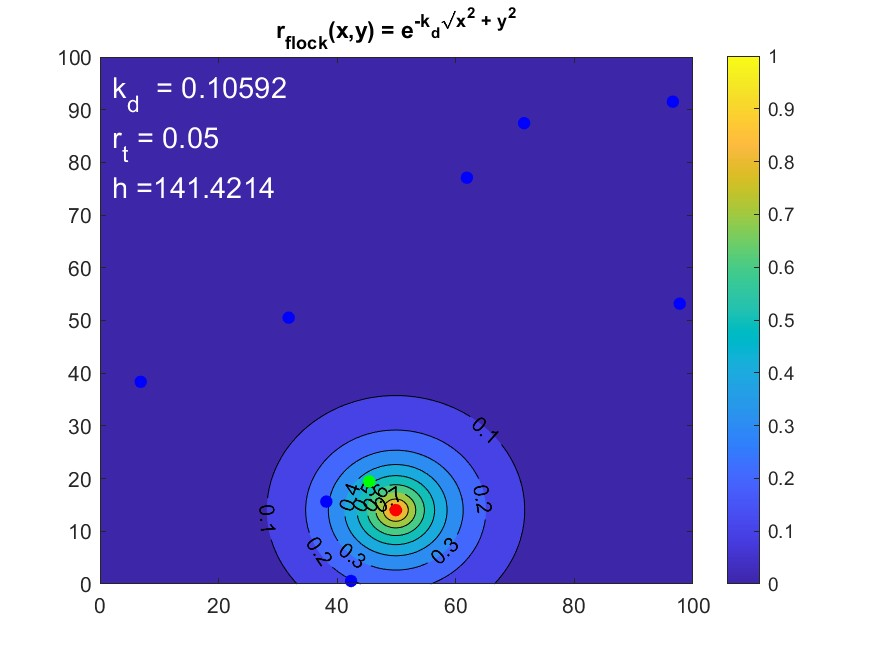
\includegraphics[width=0.7\linewidth]{figures/DroneByItself.jpg}
    \caption{Reward for endpo}
    \label{fig:my_label}
\end{figure}


\subsubsection{Endpoint Reward}
\begin{figure}[h]
    \centering
    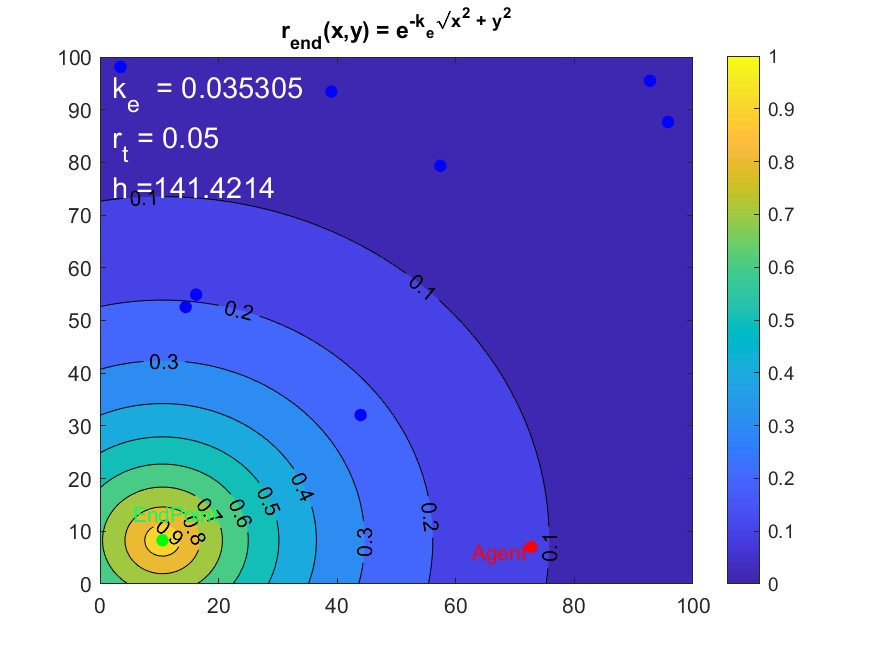
\includegraphics[width=0.7\linewidth]{figures/EndByitself.jpg}
    \caption{Caption}
    \label{fig:my_label}
\end{figure}
\clearpage

\subsubsection{Individual reward function for 9 drones}

\begin{figure}[h]
    
    \centering
   \begin{subfigure}[b]{0.3\textwidth}
         \centering
         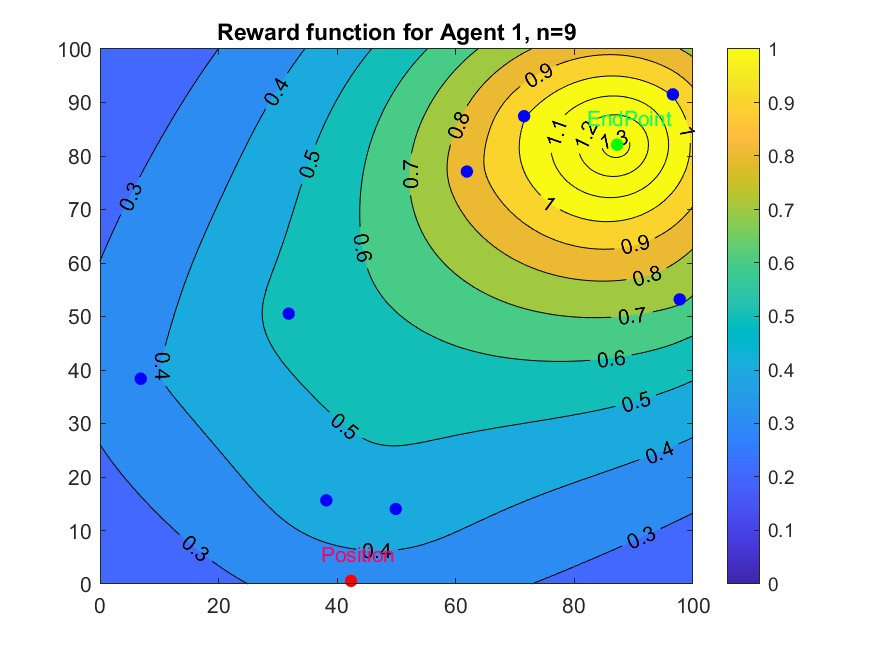
\includegraphics[width=\textwidth]{figures/RewardFunction1.jpg}
         \caption{Drone 1}
         \label{fig:r1}
     \end{subfigure}
     \hfill
     \begin{subfigure}[b]{0.3\textwidth}
         \centering
         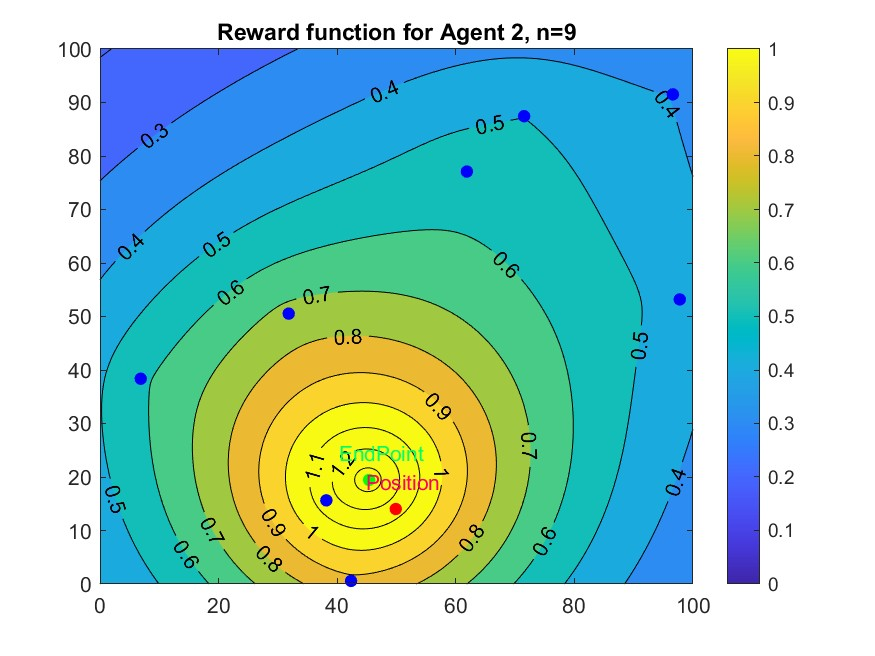
\includegraphics[width=\textwidth]{figures/RewardFunction2.jpg}
         \caption{Drone 2}
         \label{fig:r2}
     \end{subfigure}
     \hfill
     \begin{subfigure}[b]{0.3\textwidth}
         \centering
         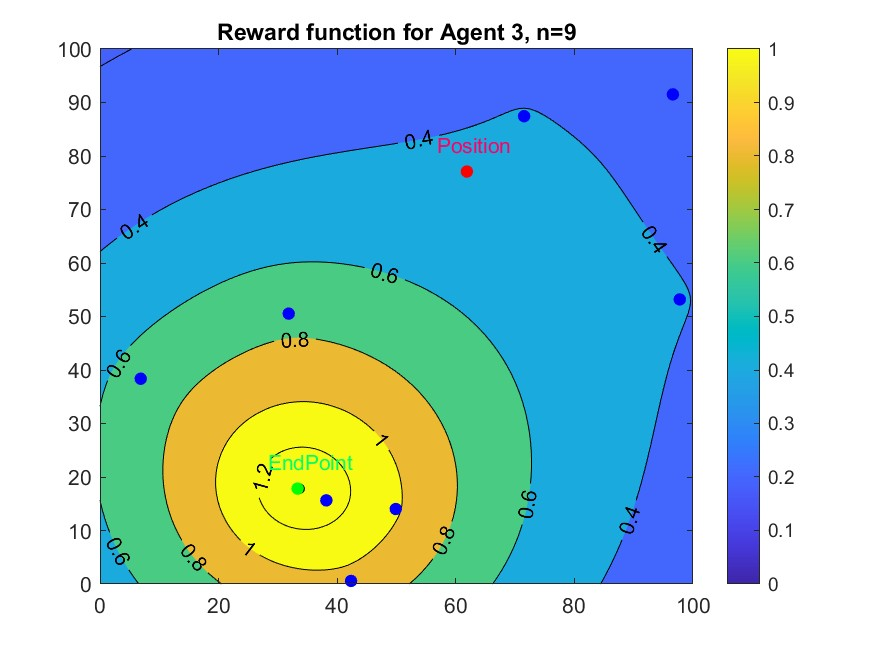
\includegraphics[width=\textwidth]{figures/RewardFunction3.jpg}
         \caption{Drone 3}
         \label{fig:r3}
     \end{subfigure}
        \begin{subfigure}[b]{0.3\textwidth}
         \centering
         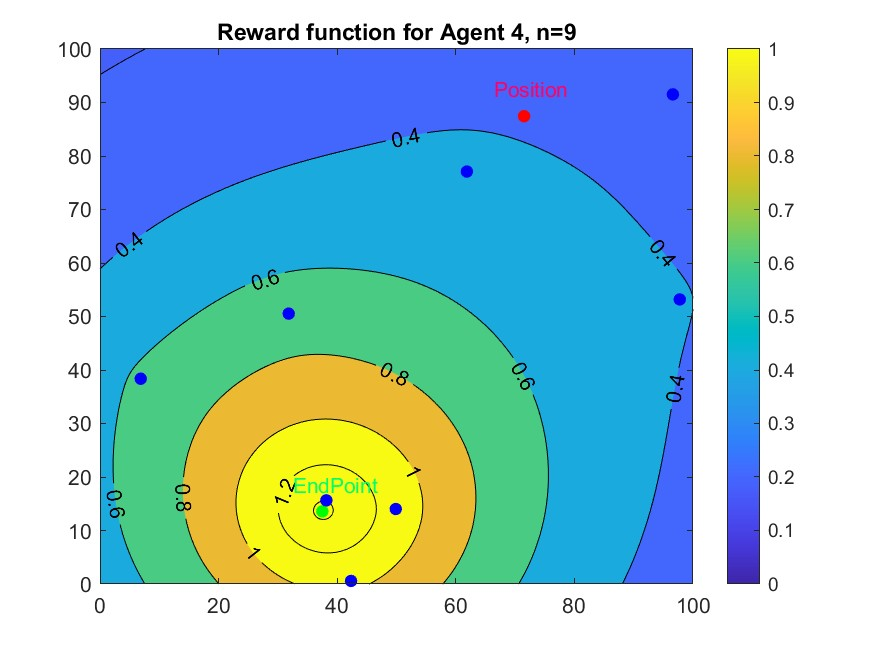
\includegraphics[width=\textwidth]{figures/RewardFunction4.jpg}
         \caption{Agent 4}
         \label{fig:r4}
     \end{subfigure}
     \hfill
     \begin{subfigure}[b]{0.3\textwidth}
         \centering
         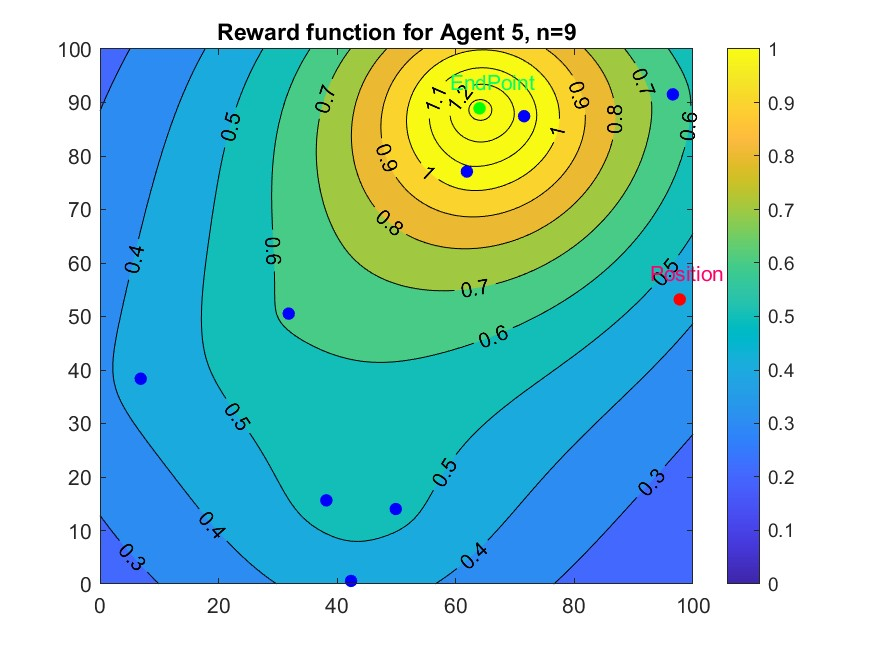
\includegraphics[width=\textwidth]{figures/RewardFunction5.jpg}
         \caption{Agent 5}
         \label{fig:r5}
     \end{subfigure}
     \hfill
     \begin{subfigure}[b]{0.3\textwidth}
         \centering
         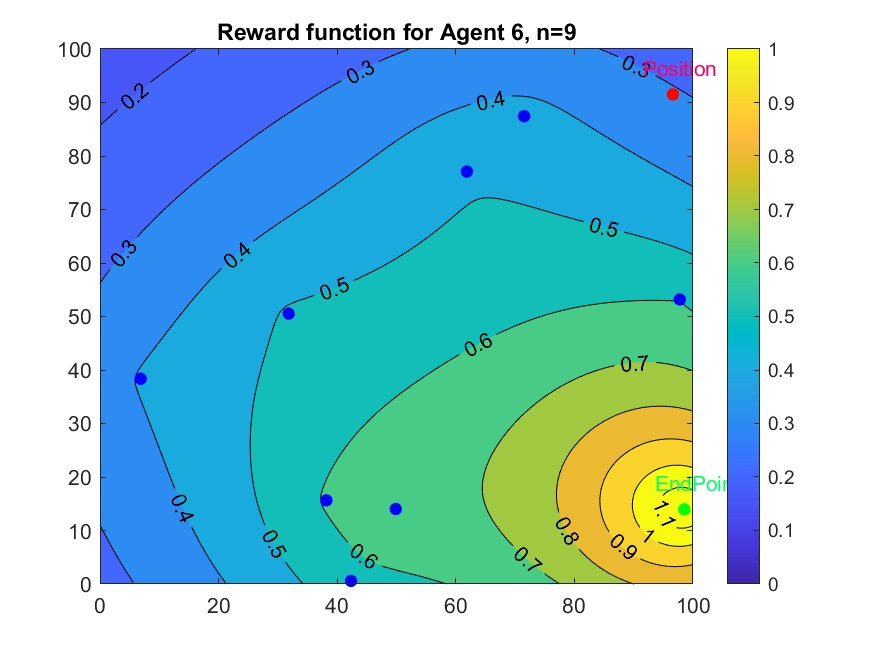
\includegraphics[width=\textwidth]{figures/RewardFunction6.jpg}
         \caption{Drone 6 reward function}
         \label{fig:r6}
     \end{subfigure}
        \begin{subfigure}[b]{0.3\textwidth}
         \centering
         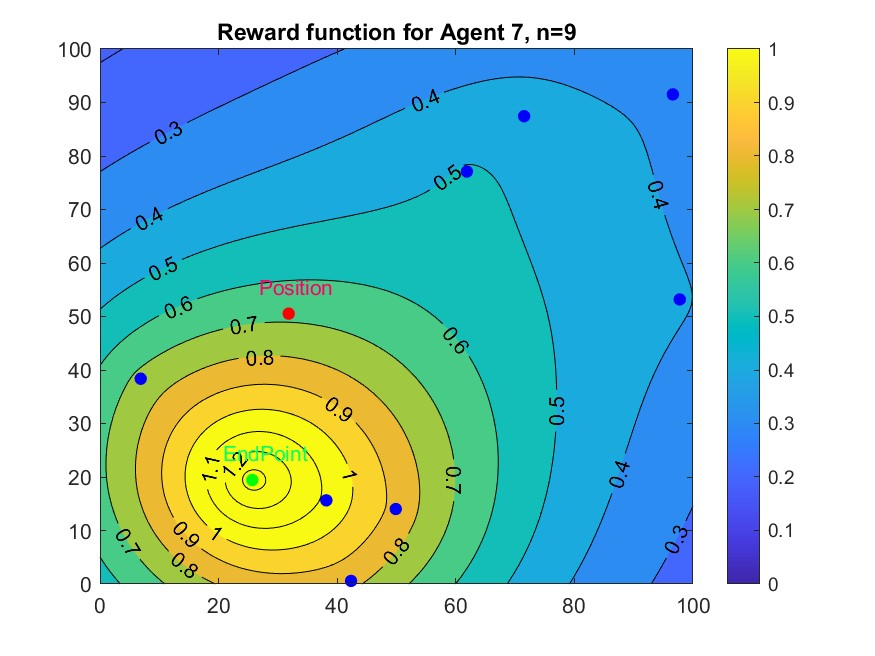
\includegraphics[width=\textwidth]{figures/RewardFunction7.jpg}
         \caption{Agent 7}
         \label{fig:r7}
     \end{subfigure}
     \hfill
     \begin{subfigure}[b]{0.3\textwidth}
         \centering
         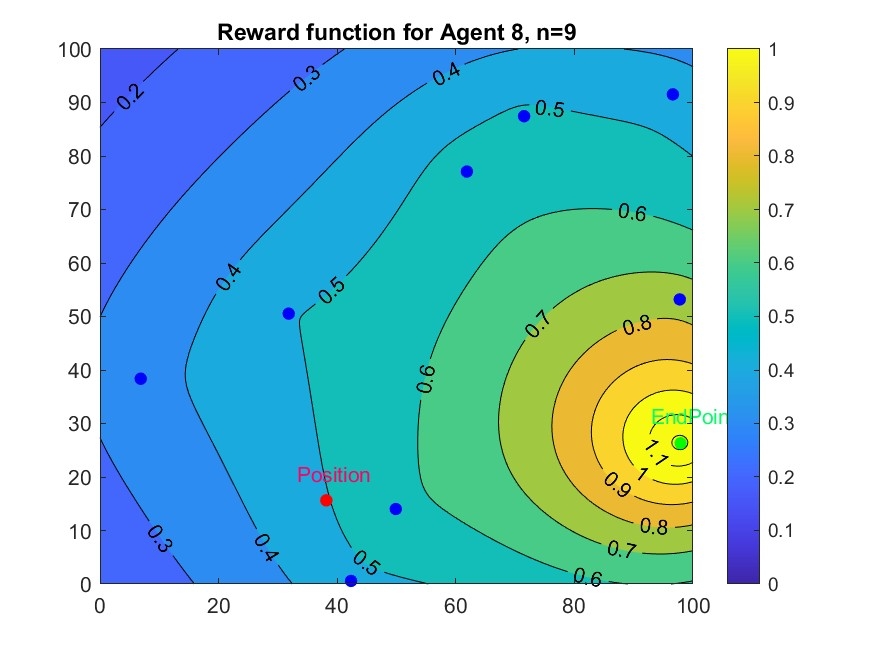
\includegraphics[width=\textwidth]{figures/RewardFunction8.jpg}
         \caption{Agent 8}
         \label{fig:r8}
     \end{subfigure}
     \hfill
     \begin{subfigure}[b]{0.3\textwidth}
         \centering
         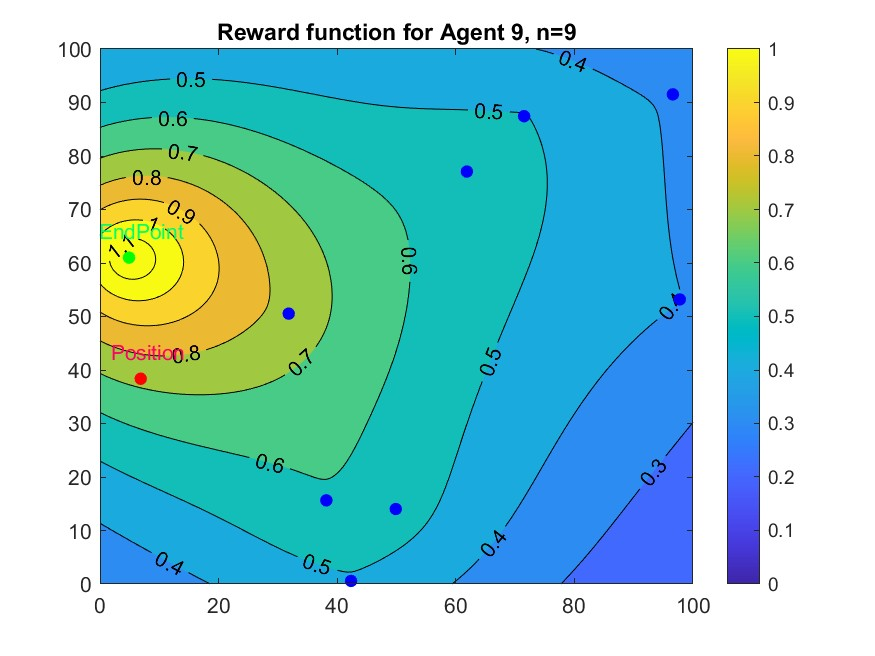
\includegraphics[width=\textwidth]{figures/RewardFunction9.jpg}
         \caption{Agent 9}
         \label{fig:r9}
     \end{subfigure}
        \caption{Reward functions for 9 different Agents}
        \label{fig:three graphs}
   
\end{figure}
\clearpage
\subsubsection{Scaling reward function relative to number of agents}
Comparison of reward function with no scaling relative to number of entities:
\begin{figure}[h]
\centering
   \begin{subfigure}[b]{0.43\textwidth}
         \centering
         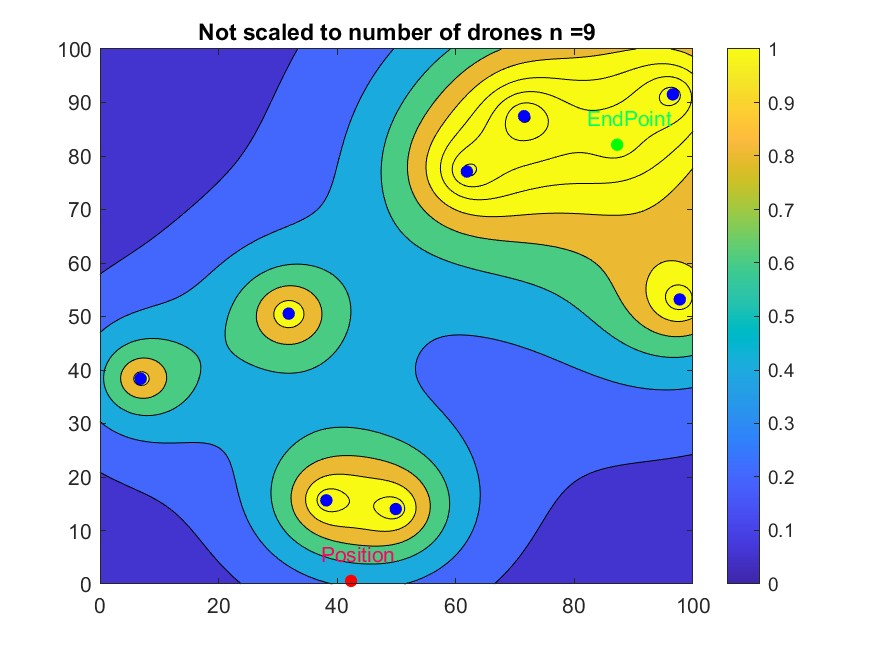
\includegraphics[width=\textwidth]{figures/RewardFunctionNotscaled9.jpg}
         \caption{Not scaled n = 9}
         \end{subfigure}
         \begin{subfigure}[b]{0.43\textwidth}
         \centering
         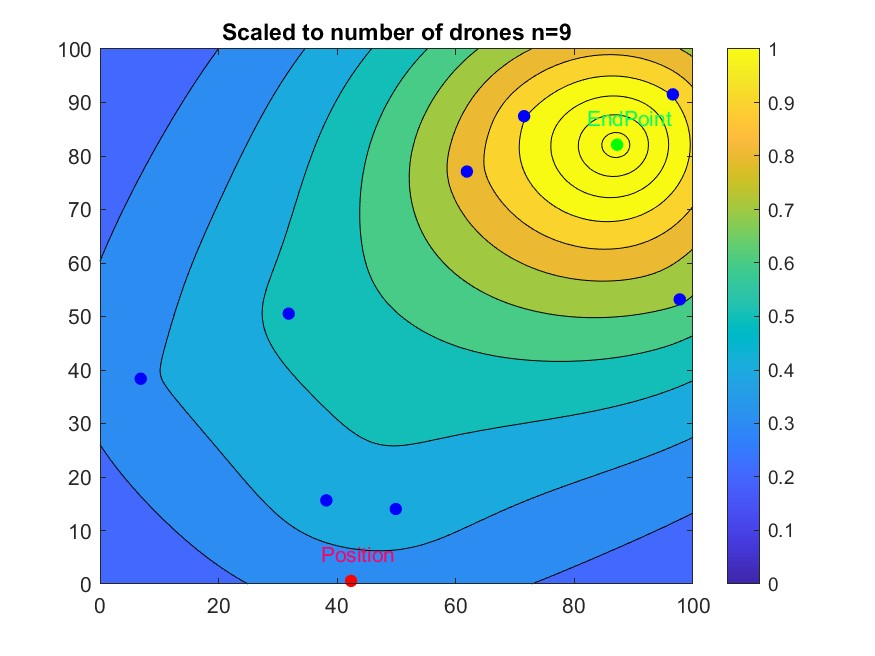
\includegraphics[width=\textwidth]{figures/RewardFunctionscaled9.jpg}
         \caption{Scaled n = 9}
         \end{subfigure}
         \hfill 
         \begin{subfigure}[b]{0.43\textwidth}
         \centering
         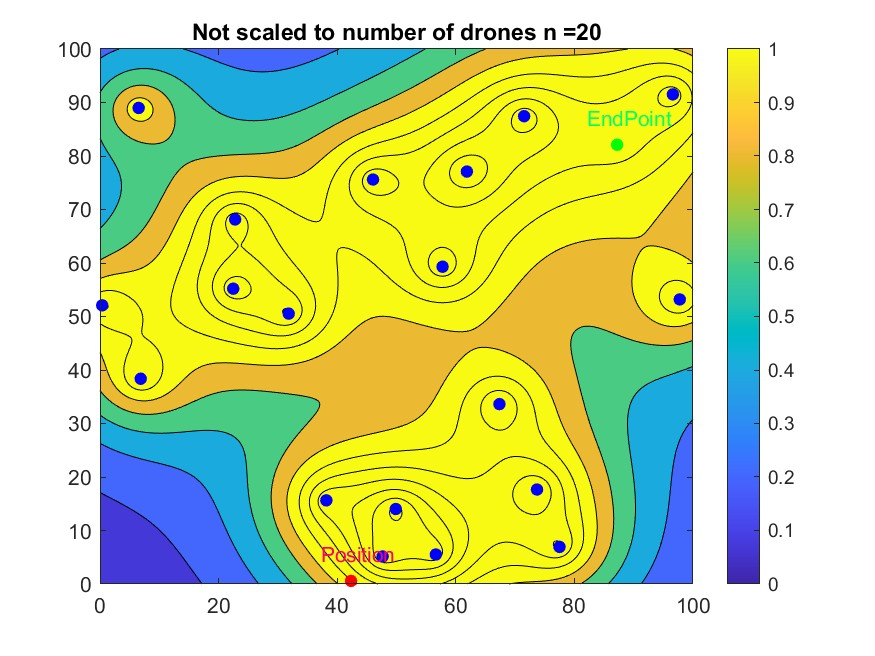
\includegraphics[width=\textwidth]{figures/RewardFunctionNotscaled20.jpg}
         \caption{Not scaled n = 20}
         \end{subfigure}
         \begin{subfigure}[b]{0.43\textwidth}
         \centering
         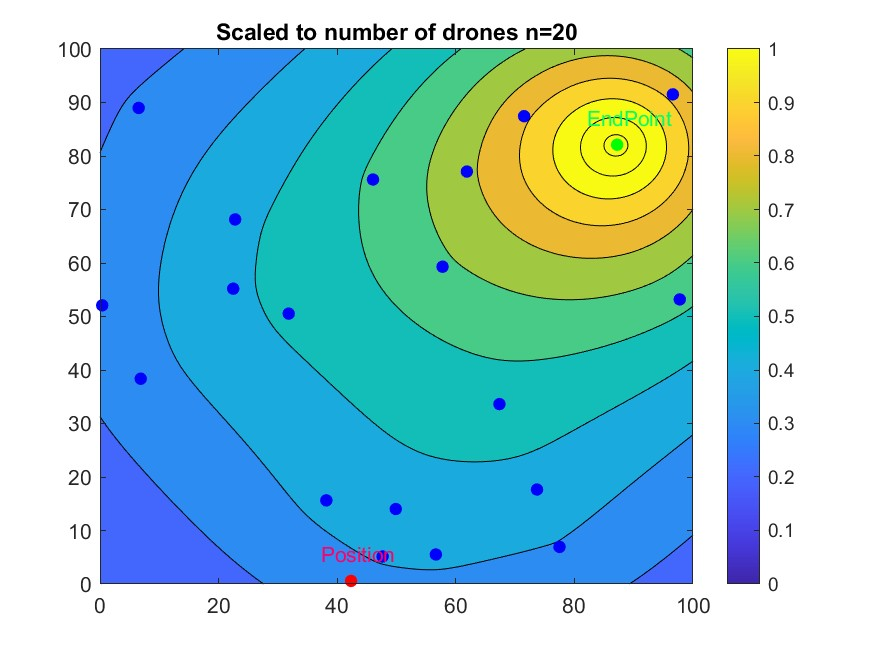
\includegraphics[width=\textwidth]{figures/RewardFunctionscaled20.jpg}
         \caption{Scaled n = 20}
         \end{subfigure}
         \hfill
          \begin{subfigure}[b]{0.43\textwidth}
         \centering
         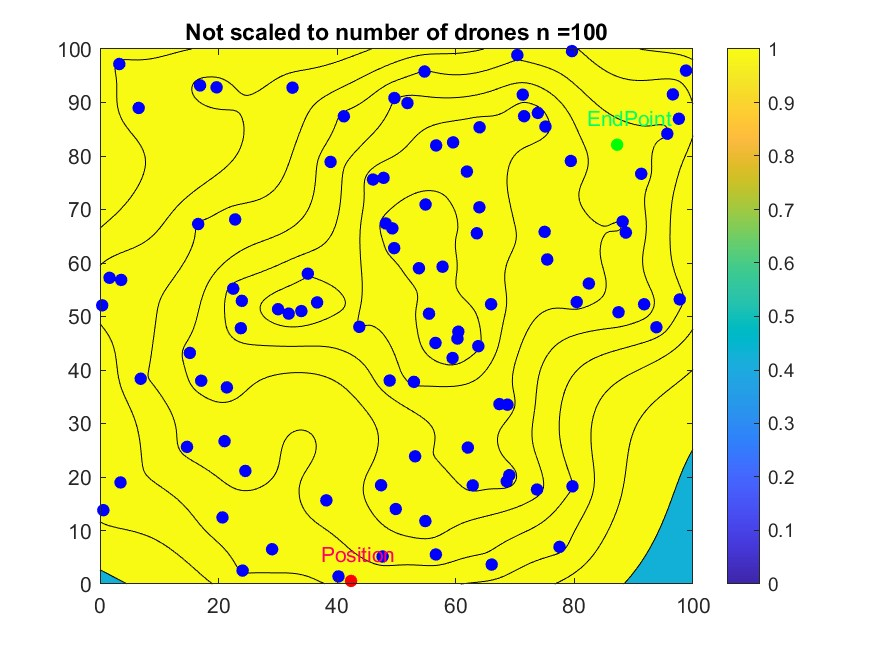
\includegraphics[width=\textwidth]{figures/RewardFunctionNotscaled100.jpg}
         \caption{Not scaled n = 100}
         \end{subfigure}
         \begin{subfigure}[b]{0.43\textwidth}
         \centering
         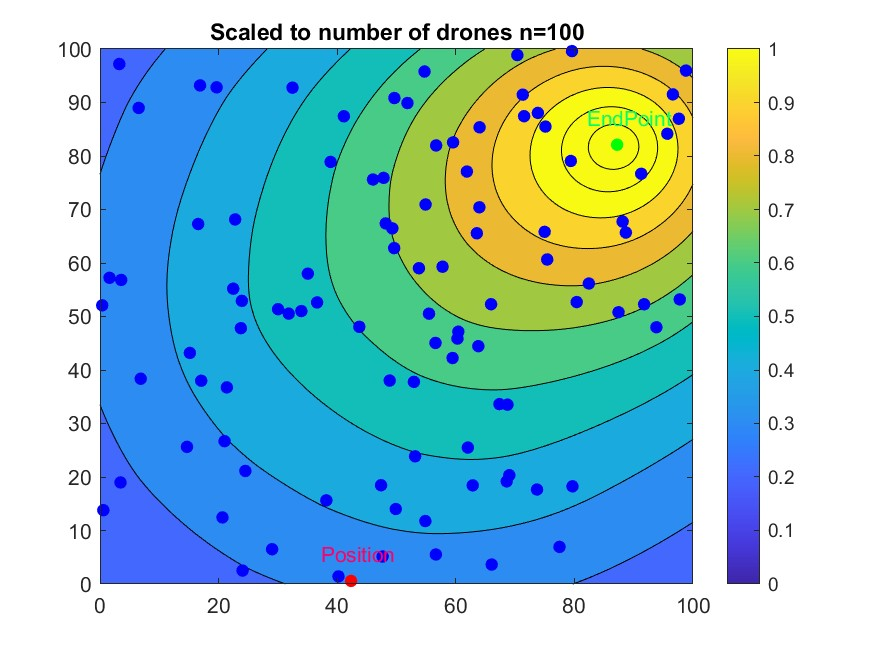
\includegraphics[width=\textwidth]{figures/RewardFunctionscaled100.jpg}
         \caption{Scaled n = 100}
         \end{subfigure}
\end{figure}